\clearpage
\newgeometry{margin=1cm}
\thispagestyle{empty}
\begin{landscape}
\begin{table}[t!]
\caption{Cost of safety guarantees}
\label{tbl-safety-cost}
    \begin{tabular}{lrrrrrrrrrrrrrrr} % UPDATED 20180305
    \toprule
                                        & B.sort     &  H.sort    & Bin.Search & XXTEA      & MD5        & RC5        & FFT        & Outlier    & LEC        & CoreMark   & MoteTrack  & HeatCalib  & HeatDetect & \makebox[0.2mm]{} &   average \\
    \midrule
    \midrule
    \multicolumn{10}{l}{EXECUTED BYTECODE INSTRUCTIONS (\% of total executed bytecode instructions)} \\
    Array element/object field STORES   &       18.0 &        7.8 &        0.0 &        2.9 &        4.5 &        1.5 &        6.1 &        5.8 &        3.7 &        2.6 &       10.0 &        1.4 &        4.7 &                   &       5.3 \\
    Array element/object field LOADS    &       18.0 &       15.9 &        7.1 &        8.6 &        6.2 &        6.4 &        7.0 &       10.7 &        7.9 &       11.6 &       21.4 &        4.1 &        9.8 &                   &      10.4 \\
    \multicolumn{10}{l}{PERFORMANCE OVERHEAD VS NATIVE C (\% of native C)} \\
    unsafe                              &      101.2 &       88.5 &       65.2 &       57.6 &       45.7 &       19.5 &       17.7 &       75.7 &       84.6 &       97.0 &      156.3 &       30.5 &       73.4 &                   &      70.2 \\
    safe writes                         &      247.5 &      153.9 &       65.2 &       68.2 &       60.3 &       22.2 &       30.3 &      128.4 &      118.4 &      124.0 &      266.1 &       33.9 &       91.3 &                   &     108.4 \\
    safe reads and writes               &      393.9 &      287.8 &      151.7 &      100.0 &       80.3 &       33.4 &       43.0 &      226.6 &      179.8 &      202.2 &      445.1 &       43.9 &      126.9 &                   &     178.0 \\
    \multicolumn{10}{l}{PERFORMANCE OVERHEAD VS UNSAFE VM (\% of unsafe AOT)} \\
    safe writes                         &       72.7 &       34.7 &        0.0 &        6.7 &       10.0 &        2.3 &       10.7 &       30.0 &       18.3 &       13.7 &       42.8 &        2.6 &       10.3 &                   &      22.4 \\
    safe reads and writes               &      145.5 &      105.7 &       52.4 &       26.9 &       23.7 &       11.6 &       21.5 &       85.9 &       51.6 &       53.4 &      112.7 &       10.3 &       30.9 &                   &      63.3 \\
    \multicolumn{10}{l}{CODE SIZE OVERHEAD VS NATIVE C (\% of native C)} \\
    unsafe                              &      118.6 &      100.0 &      112.3 &       55.1 &       54.9 &      121.8 &        2.5 &      110.5 &       88.6 &       50.7 &      117.1 &      -17.2 &      107.7 &                   &      78.7 \\
    safe writes                         &      125.4 &      105.4 &      112.3 &       56.2 &       55.7 &      125.3 &        5.0 &      118.9 &       94.3 &       54.5 &      125.4 &      -16.4 &      114.7 &                   &      82.8 \\
    safe reads and writes               &      132.2 &      113.4 &      117.8 &       60.1 &       59.1 &      132.3 &        8.0 &      123.2 &      102.9 &       61.8 &      145.3 &      -13.9 &      118.5 &                   &      89.3 \\
    \multicolumn{10}{l}{CODE SIZE OVERHEAD VS UNSAFE VM (\% of unsafe AOT)} \\
    safe writes                         &        3.1 &        2.7 &        0.0 &        0.7 &        0.5 &        1.6 &        2.4 &        4.0 &        3.0 &        2.5 &        3.8 &        1.0 &        3.4 &                   &       2.3 \\
    safe reads and writes               &        6.2 &        6.7 &        2.6 &        3.2 &        2.7 &        4.7 &        5.4 &        6.0 &        7.6 &        7.4 &       13.0 &        4.0 &        5.2 &                   &       5.9 \\
    \bottomrule
    \end{tabular}
\end{table}
\end{landscape}
\clearpage
\restoregeometry


\section{The cost of safety}
\label{sec-evaluation-safety}

The advantage of using a VM to provide safety is that the necessary checks are easy to do, compared to native code, and most can be done at translation time. This leads to both a very modest increase in VM complexity due to the safety checks, and a lower run-time overhead. 
% would be nice to get code size for Harbor and t-kernel.

\subsection{Run-time cost}
\label{sec-evaluation-run-time-cost}

\begin{figure}
\centering
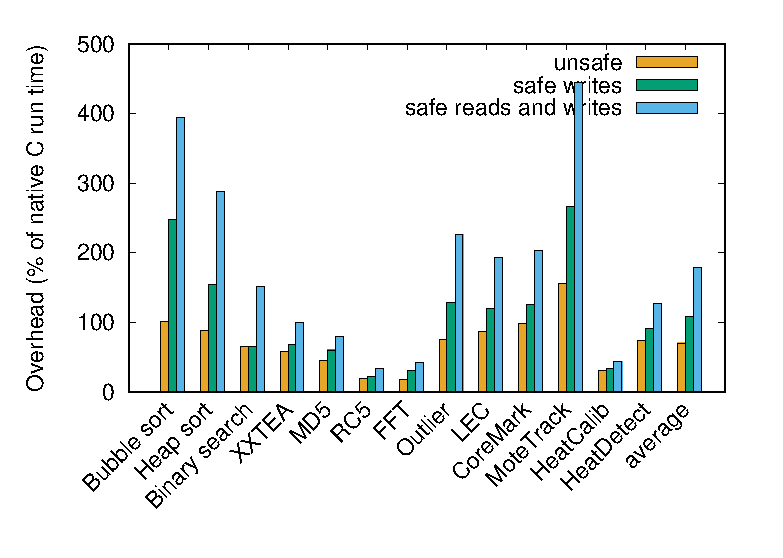
\includegraphics[width=\mygraphsize]{safety-cost.eps}
\caption{Overhead increase due to safety checks}
\label{fig-safety-cost-per-benchmark}
\end{figure}

\begin{figure}
\centering
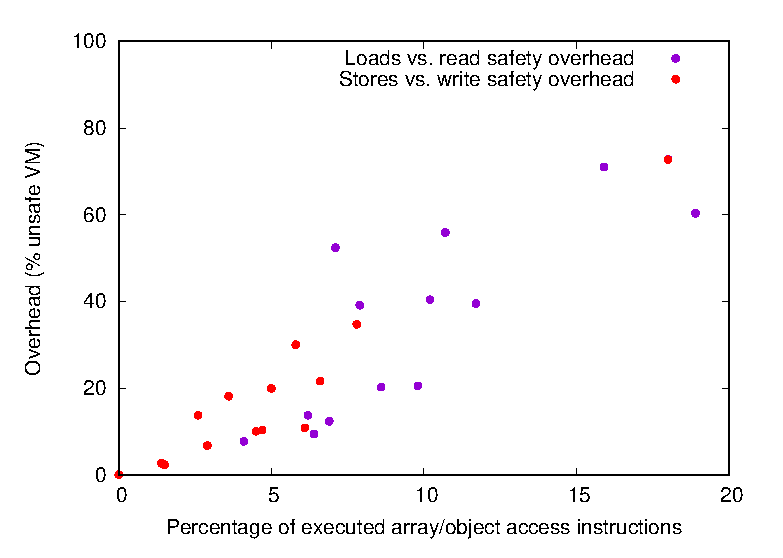
\includegraphics[width=\mygraphsize]{safety-ld-st-percentage-vs-overhead.eps}
\caption{Percentage of array/object load/store instructions and cost of read/write safety}
\label{fig-safety-ld-st-percentage-vs-overhead}
\end{figure}

\begin{figure}
\centering
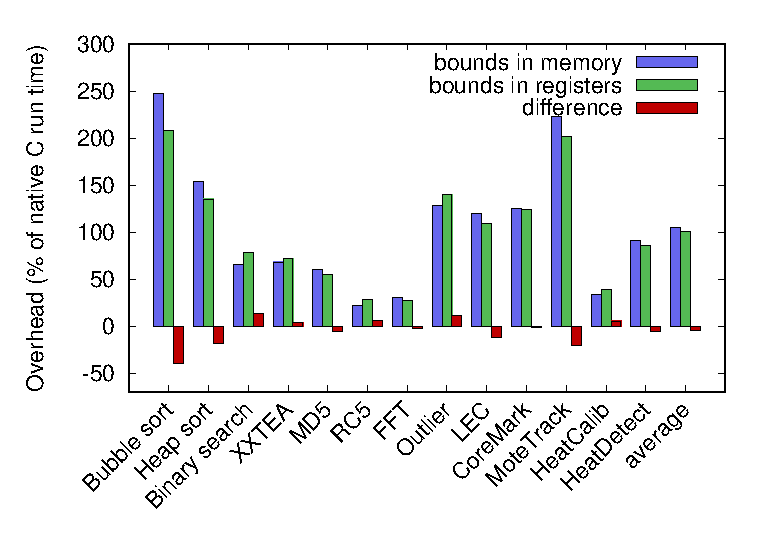
\includegraphics[width=\mygraphsize]{safety-cost-diff-using-regs.eps}
\caption{Comparison of safety cost with heap bounds in memory or registers}
\label{fig-safety-cost-memory-or-registers}
\end{figure}

Table \ref{tbl-safety-cost} shows the increase in performance and code size overhead as a result of the run-time safety checks for our 12 benchmarks. Figure \ref{fig-safety-cost-per-benchmark} shows performance overhead for both the unsafe and safe versions of the VM. The baseline here is the unsafe version of our VM, which is on average 71.1\% slower than native C. Adding write checks is sufficient to satisfy our guarantee that no malicious code can corrupt the state of the VM. This increases the average overhead to 105.3\% of native C, corresponding to an 19.9\% increase in run time compared to the unsafe VM.

The cost of the run-time safety checks depends greatly on the benchmark we run. Most checks are done at translation time, including writes to local and static variables. The only check that adds significant run-time overhead is check \ref{chk-memory-access-within-heap}, which checks the target of an object field or array write is within the bounds of the heap.

Thus, the run-time overhead is determined by the number of object or array accesses a benchmark does. The percentage of these is shown in the first part of Table \ref{tbl-safety-cost}. Since \mybench{bubble sort} has by far the highest percentage of array writes, at 18\% of all executed bytecode instructions, it also incurs the highest overhead from adding write safety, and slows down by 47\%. \mybench{Binary search} on the other hand, which does no writes at all, is unaffected. As usual \mybench{CoreMark}, being a large benchmark with a mix of operations, is somewhere in the middle. The correlation between the percentage of array and object writes, and the slowdown compared to the unsafe version is shown in Figure \ref{fig-safety-ld-st-percentage-vs-overhead}.

\subsubsection{Safe reads}
Next we consider read safety. Up to this point the VM only checks the application cannot \emph{write} to memory it's not supposed to write to, however, it may still read from any location.

The recently published Meltdown and Spectre vulnerabilities in desktop CPUs can be exploited by malicious code to read from anywhere in memory, exposing both kernel's and other applications private data, which may contain sensitive information such as authentication tokens, passwords, etc. This sent OS vendors rushing to release patches, which early report suggest may cause a performance penalty of up to 11\% \cite{Simakov:2018wp}.

Whether this is also a problem on a sensor node depends on the scenario. If the VM or other tasks contain sensitive information, then this may need to be protected. However, in many sensor node applications the node may only be running a single application, and the VM does not contain any state that would be useful to an attacker. In these cases, only providing write safety will be sufficient.

Adding read safety to our VM is trivial: instructions to load local and static variables are already protected since they use the same code to access a variable as the store instructions. For heap access, we simply add the same call to \mycode{heapcheck} to the \mycode{GETARRAY} and \mycode{GETFIELD} instructions just before the actual read.

Figure \ref{fig-safety-cost-per-benchmark} shows the cost of providing read safety is higher than write safety. Most applications read from an array or object much more frequently than they write to them. As a result, our VM with read and write safety turned on slows down by 60\% on average, corresponding to a 174\% slowdown over native C. In addition to the sort benchmarks, \mybench{MoteTrack} also suffers greatly from adding read safety, since it spends 19\% of it's instructions reading from the complex RSSI signature data structure. \mybench{RC5} is the fastest benchmark, since it not only does relatively few array reads and writes, but also spends a large amount of time on expensive variable bit shifts, which have identical performance in both C and AOT compiled versions. The result is a slowdown of only 33\% compared to native C for the fully safe version.

\subsubsection{Keeping heap bounds in registers}
In Section \ref{sec-safety-heap-access} several alternatives for the heap bounds check were considered, one of which was to keep the bounds in dedicated registers to avoid having to fetch them from memory for each check. Here we evaluate this choice.

Having the bounds in registers would reduce the cost of the check from 22 to 14 cycles, reducing the overhead of safety checks by $8/22 \approx 36\%$. However, this uses 4 registers which we can't use for stack caching.

To estimate the performance of this approach, the benchmarks were run using the unsafe VM, with the number of registers available to the stack cache reduced by 4. Since this doesn't affect the number of heap accesses, we then added the observed overhead for safety checks, reduced by 36\%.

Figure \ref{fig-safety-cost-memory-or-registers} shows the overhead for our chosen approach with the heap bounds in memory, compared to the expected overhead when the heap bounds are stored in registers. For some benchmarks such as \mybench{bubble sort} and \mybench{MoteTrack}, the savings in heap bounds checks outweighs the reduced effectiveness of the stack cache. But the improvement in performance is relatively small, and for other benchmarks the reverse is true, showing minor slowdowns when heap bounds are kept in registers. On average the benchmarks are quite balanced, as is the larger \mybench{CoreMark} benchmark.

As future work we may consider using some basic statistics, such as the percentage of array write instructions and average stack depth, to choose one of the two options on a per-method basis. But as usual there is a tradeoff, in this case VM size and complexity, which may not be worth the effort given the relatively small gains.

\subsection{Code-size cost}
Next, we examine the cost of safety in terms of code size. This comes in two parts: increase VM complexity and size, and the increase in the code it generates.

Most of our checks are not more complex than comparing two integers, and failing if a condition is not met. The most complex part is deciding the stack effects of instructions to guard against stack over- or underflow. This comes in the form of a table that encodes the effects of most instructions, and some specialised code to analyse a handful of instructions without fixed effect. In total, the increase in VM size for our safe version is a modest 1776 bytes.

As we can see in Table \ref{tbl-safety-cost}, the size of the code the VM generates increases by only $(181.8/177.7)-1=2.3\%$. Since most checks occur at translation time, most instructions produce exactly the same native code in the safe version of our VM. The exceptions are \mycode{INVOKEVIRTUAL} and \mycode{INVOKEINTERFACE}, which now contain the expected stack effects to realise check \ref{chk-invokevirtual-stack-effects-match}, and the array and object write instructions \mycode{PUTFIELD} and \mycode{PUTARRAY}, that emit a single extra \mycode{CALL} instruction the \mycode{heapcheck} routine. Since these instructions are both relatively rare, and already generate a relatively large block of native instructions, the total effect on code size is very limited.

\subsection{Comparison to native code alternatives}
As discussed in Section \ref{sec-state-of-the-art-safety}, several non-VM approaches have been proposed to guarantee safety on a sensor node. Two of these, \emph{t-kernel} and Harbor, allow the node to guarantee safety independent of the host. In this section we compare these to our approach, and consider the question whether a VM is a good way to provide safety.

\emph{t-kernel} reports a slowdown of between 50 and 200\%, which is roughly in the same range as our VM. However both \emph{t-kernel} and our approach provide additional advantages. In \emph{t-kernel}'s case a form of virtual memory, and for our VM platform independence. This makes them hard to compare, but we note that while the performance of both systems is similar, \emph{t-kernel}'s code size overhead is much larger at a 6-8.5x increase, limiting the size of programmes we can load onto the device.

A better comparison is possible for Harbor, which only provides safety. The overhead reported is in the range of 160 to 1230\%. The latter is for a synthetic benchmark, filling a block of memory with arbitrary data. The authors claim this simulates a common behaviour of sensor network applications: copying sampled sensor data into a buffer that can be transmitted into the network.

We implemented this as a benchmark that fills an array of 256 elements with an arbitrary number. This is one of the worst cases for our safe VM since consecutive array writes are expensive for two reasons: (i) in our VM this results in repeated executions of the \mycode{PUTARRAY} instruction, which calculates the target address for each write, while native code can slide a pointer over the array, and (ii) each of these writes will trigger a call to \mycode{heapcheck}.

Our benchmark is implemented as a simple loop as shown in Listing \ref{lst-fill-array}.

\begin{listing}
\begin{minted}{java}
    for (short i = 0; i < NUMBERS; i++) {
        numbers[i] = (byte)1;
    }
\end{minted}
\caption{Fill array benchmark (8-bit version)}
\label{lst-fill-array}
\end{listing}

% UPDATED 20180213

\begin{table}[]
 \centering
 \caption{Overhead for the fill array benchmark as a percentage of native C}
 \label{tbl-fill-array-results}
\begin{tabular}{lrrr}
\toprule
%benchmark & unsafe overhead & safe overhead \\
%\midrule
%8-bit  byte  & 210\% & 566\% \\
%16-bit short & 182\% & 452\% \\
%32-bit int   & 155\% & 336\% \\
Benchmark & Unsafe & Safe & Increase due to \\
 & overhead & overhead & safety checks \\
\midrule
8-bit  bytes  & 210.1\% & 566.4\% & 356.3\% \\
16-bit shorts & 182.8\% & 451.5\% & 268.7\% \\
32-bit ints   & 155.3\% & 335.6\% & 180.3\% \\
\bottomrule
\end{tabular}
\end{table}


The resulting overhead is shown in Table \ref{tbl-fill-array-results}. We implemented our benchmark for arrays of bytes, shorts and ints. Unfortunately the Harbor paper does not mention the size of elements in their buffer, nor how this would affect their overhead. For our VM, the worst case is filling a byte array because here the relative overhead from address calculation and safety checks is highest.

The worst case extra overhead due to safety checks is 356\% of the native C execution time, considerably less than Harbor. This drops to 180\% when storing ints instead of bytes. In addition, our VM also incurs overhead not related to safety checks, but the total overhead of 566\% in the worst case is still less than half of Harbor's 1230\%.

While our VM is currently faster than Harbor, the comparison is not entirely fair. Harbor lists the cycle overhead for all of it's 5 run-time protection primitives. We assume that without any function calls, only the 'Write access check' is relevant to this benchmark, which takes 65 cycles. In contrast, our \mycode{heapcheck} routine only takes 22 cycles.

The difference is due to Harbor's more fine grained protection, which allows it to grant access to any aligned block of 8 bytes to the application, while our VM's protection is more coarse. If Harbor could be modified to use a check similar to ours, it's overhead could potentially be reduced to $1230 / 65 * 22 \approx 416\%$. This puts it in the middle of our three versions in terms of total overhead. However, it is not clear from the paper whether Harbor's architecture could support such a coarse-grained check since it requires all application data that needs run-time write checks to be in a single segment.

While this shows our approach achieves a performance comparable to even an optimised version of Harbor, it does not highlight the advantage of using a VM to provide safety since both approaches must check each write to the array. However, our approach can verify writes to local and static variables to be safe at translation time, eliminating the need for a run-time check, while we can tell from the Harbor sources \cite{sos-operating-system} that its verifier requires \emph{all} stores to go through the write access check. The authors do note that static analysis of the code could reduce the number of checks, but that this would come at the cost of a significantly more complex verifier.

This means our approach should have a distinct advantage for code with more frequent writes to local variables. The Harbor paper also contains an FFT benchmark, and we use the same code from the Harbor sources for our \mybench{FFT} benchmark. In Harbor's case this results in an overhead of 380\%. Even with the faster memory access check, the overhead would be $380 / 65 * 22 \approx 129\%$, while our VM is significantly faster at only 30.4\%.
